
% to choose your degree
% please un-comment just one of the following
\documentclass[bsc,frontabs,twoside,singlespacing,parskip,deptreport]{infthesis}     % for BSc, BEng etc.
% \documentclass[minf,frontabs,twoside,singlespacing,parskip,deptreport]{infthesis}  % for MInf


\usepackage{graphicx}
\usepackage{caption}
\usepackage{subcaption}
\begin{document}

\title{Implementing an online open-source prediction market framework}

\author{Yordan Stoyanov}

% to choose your course
% please un-comment just one of the following
%\course{Artificial Intelligence and Computer Science}
%\course{Artificial Intelligence and Software Engineering}
%\course{Artificial Intelligence and Mathematics}
%\course{Artificial Intelligence and Psychology }   
%\course{Artificial Intelligence with Psychology }   
%\course{Linguistics and Artificial Intelligence}    
%\course{Computer Science}
\course{Software Engineering}
%\course{Computer Science and Electronics}    
%\course{Electronics and Software Engineering}    
%\course{Computer Science and Management Science}    
%\course{Computer Science and Mathematics}
%\course{Computer Science and Physics}  
%\course{Computer Science and Statistics}    

% to choose your report type
% please un-comment just one of the following
%\project{Undergraduate Dissertation} % CS&E, E&SE, AI&L
%\project{Undergraduate Thesis} % AI%Psy
\project{4th Year Project Report}

\date{\today}

\abstract{
Model aggregation, markets, prediction markets.

My market
}

\maketitle

\section*{Acknowledgements}
You guys have been a great inspiration!

\tableofcontents

%\pagenumbering{arabic}


\chapter{Introduction}

Information has been traded extensively in one way or another since the dawn of man. While true, this fact has become increasingly relevant in recent years with advances such as the information economy and big data transforming the way we think about data and the knowledge it implies \cite{mcgee_managing_1993}; at the same time it has never been harder to quantify its value.


The problem of efficiently combining information coming from different sources in order to form a rational belief is largely an unsolved issue in Bayesian philosophy \cite{greene_collective_2010}. It manifests in the domain of machine learning as the problem of belief aggregation which deals with the design of algorithms that combine the beliefs of multiple learners in order to elicit a more reliable prediction. In practice though existing solutions are far from ideal in the sense that they do not provide flexible enough methods of combining the different beliefs of different (heterogeneous) sources into a uniform output. 

    If we take a look at ordinary commodity trading though it is apparent that the existence of a market where agents exchange goods using a common currency provides a meaningful way to determine the prices of the traded goods. Note that while the traded goods can be physical, it is often the case that they are purely conceptual. For example the prices of stock market shares reflect the public's expectation of the performance of a company in the near future. The basic market needs not be active with regard to the traded goods and is in principle nothing more than the market squares that have existed in towns for ages. In its essence a market provides the basic process for determining the price and ownership of the various goods or services exchanged within the market.

    Prediction markets are a special kind of markets which allow agents to trade on and share their information on future events with the public. This is achieved by creating a market where the trading goods are akin to shares corresponding to each of the possible outcomes of the events of interest. Each share promises a fixed payment in the future to its holder if and only if the outcome associated with it happens to be the event's actual result. This future point is usually fixed at the start of each challenge, necessarily after the result of the event has been observed by the public. In such a way players are incentivised to trade on the difference between their beliefs and those of the market: rational agents would buy shares at what they perceive to be a lower price as this increases their expected profit. In practice by doing so they affect the instantaneous price of each of the goods and thus inform the market and the public of their knowledge. 

	
[TODO: application -> machine learning]

    Another possible application of prediction markets deals with the creation of crowdsourced machine learning competitions. Such challenges have become increasingly popular thanks in large to the fact that they leverage the expertise and knowledge of the public at scale. A prominent example is the {\em Netflix Prize} challenge which was held as early as 2006 with the goal of improving the movie classification algorithms used by the company of the same name \cite{bennett_netflix_2007}. The contest ended 3 years later with success, the winning algorithm achieving a significant improvement of over 10\% increase in the RMSE metric in comparison to the original solution \cite{koren_bellkor_2009}. The online platform {\em Kaggle} which appeared shortly afterwards takes a slightly different approach by instead hosting such crowdsourced machine learning competitions on the behalf of third parties. It has proved similarly successful, attracting an active community of data scientists from different domains and leading to improvements in the {\em state-of-the-art} algorithms used across a number of disciplines such as Biology \cite{bentzien_crowd_2013} and Physics \cite{harvey_observing_2014}. 

    Although fairly successful, this competitive approach to crowdsourcing machine learning problems exhibit a number of notable shortcomings. Most notably such challenges are inherently anti-collaborative as they incentivise participating players to keep their solutions private, in order to compete for the first places. This is a direct consequence of the reward structure which promises incentives exclusively for the top teams (or even team), and thus leads to an equilibrium where the entry requirements are constantly increasing thus effectively discouraging new players from participating - even those who possess knowledge unique to the market. 

    My project deals with the implementation of a flexible online prediction and machine learning market framework. In contrast to existing solutions modelling simple prediction markets, the software I built is intended as a extensible base for the future use of such markets in the domain of machine learning. 

To this end the software offers a concise, well-tested and documented prediction market core with a modular architecture which allows for the creation and experimental comparison of different pricing algorithms. Being a web platform it has a full-featured though fairly unsophisticated human-friendly user interface, but also includes a comprehensive market API which permits and encourages algorithmic trading. 

	While the original project topic: 
   
   
   
\chapter{Definitions}

    In this section I outline existing approaches to the problem of model aggregation, introduce the concept of prediction markets, and finally talk about their use in a machine learning context. 
% Define markets, prediction markets. Detail how we use them to aggregate beliefs.


\section{Model Aggregation}
    In machine learning the problem of model or belief aggregation deals with the design of meta-algorithms that use a number of existing classifiers for a specific task in order to elicit a more accurate prediction than any of the constituent algorithms. Such algorithms are called {\em ensemble methods} [TODO: few more sentences about ensemble methods, examples]

\section{Market}

    Markets provide a common ground for the exchange of goods between different agents. Basic markets are neutral towards both the participants and the goods being traded and do not have the concept of currency which is seen as another good instead. Each of the agents has an associated {\em position} in each of the goods being traded in the market. The value of an agent's {\em position} in a good represents the amount of the good they currently possess and in general, there is no restriction on the value of the agent's position. We will distinguish between {\em long positions} where the agent has a positive holding, and {\em short positions} where the agent has a negative amount of the good.

    A basic model of such a market is the {\em order book} which records and matches the bids and offers placed by participating agents. Such a market is {\em neutral} with regard to the goods as it never owns any. Note that there is an inherent degree of freedom when implementing the matching process: arbitrage opportunities must be dealt with care if the market is to be strictly neutral, and the same goes for partially completing orders (since rarely, if ever both the price and the quantity will match).


\section{Prediction Market}

    A prediction market is a type of market with an agreed currency where each of the remaining goods is tied to exactly one of the possible outcomes of a future event. Each good promises a fixed reward (taken to be 1 credit for simplicity) in case the outcome associated with it happens to be the event's actual result, and zero otherwise. Goods can be additionally created by agents for sale, which is equivalent to the agent assuming a short position in the market. 
    
    Prediction markets have been shown to outperform other traditional forms of prediction such as public opinion polls. They have been used with success in the past for health care \cite{polgreen_use_2007}, to aid decision-taking in large corporations \cite{cowgill_using_2009}, and to predict presidential elections \cite{dudik_combinatorial_2013}. Recently prediction markets such as intrade.com were also shown to provide more accurate results on the Scottish referendum as compared to traditional voter polls \cite{bell_independence_2014}.

\section{Market Maker}
    [TODO]

\section{Machine Learning Market}
    {\bf Machine learning markets} (also {\bf artificial prediction markets}) are a fairly recent extension of the concept of prediction markets which establish parallels between prediction markets and machine learning approaches for model combination. 

In a machine learning market the players are machine learning agents possessing individual {\em utility} or {\em betting} functions in addition to defining their probabilistic beliefs. As in ordinary prediction markets the traded goods correspond to the possible outcomes of the events (or variables) of interest. An important constraint is the {\em no-arbitrage} assumption which dictates that the prices of the goods corresponding to the disjoint outcomes of an event must be well-defined and equal to the goods' payout of 1 credit. The goods' prices thus form a probability distribution over the outcome space. In practice this is achieved by the use of an {\em active} market maker that determines the current price of goods by resolving arbitrage opportunities or providing liquidity to the market. 

	Barbu and Lay introduced the concept of an {\bf artifical prediction market} as early as 2010 \cite{barbu_supervised_2010}. The concept has been later extended and published formally in 2012 \cite{barbu_introduction_2012}. In artificial prediction markets agents act according to their beliefs and a specified {\em betting function}. An important result obtained by the authors for this kind of markets is that agents with fairly simple (e.g. linear or logarithmic) betting functions generalise existing algorithms such as random forests and logistic regression and often outperform them in practice. More importantly 

	An important paper by Storkey \cite{storkey_machine_2011} introduces the concept of {\bf machine learning markets}. In contrast to the framework proposed by Barbu and Lay, agents in machine learning markets are defined by an {\em utility} function. In practice this means that agents' bets need not be strictly proportional to their current wealth. Furthermore, markets of discrete, multivariate and possibly joint outcome spaces are considered. In his paper Storkey establishes the theoretical equivalence between market dynamics observed in machine learning markets with agents of simple, fixed utility functions and existing machine learning approaches, such as mixture models (linear aggregation, product of experts) and message passing algorithms. 

[TODO] Of note is the observation that the belief functions considered under this framework require agents' bets to be strictly proportional to their total wealth, which needs not be the case for machine learning markets in general. 


\chapter{Related Software}

% I will then review some case studies of prediction markets at work. Finally I will have a look at the existing solutions that could be used as a base for my project.

%
    My search for software started first and foremost with an investigation of the open-source solutions which could be used as a starting point for my project. I then had a look at a number of closed-source or commercial prediction markets which I investigated similarly in terms of UI and functionality.   
    
\section{Open Source Projects}
    Despite the fact that prediction markets are not a particularly novel concept and are relatively well-studied I was unable to find a satisfying project which I could use as a starting point for my market. The solutions I found and examined were in general too limited in architecture, mostly outdated and built on top of aging or relatively uncommon web stacks.

\begin{itemize}

\item {\tt Zocalo}

    Zocalo is an MIT-licensed prediction market written in Java using Java Server Pages (JSP) and Hibernate. It is probably the most prominent of the listed examples having been used in a number of research projects in Economics (\cite{carver_architecture_2008}, \cite{chang_simulating_2009}. It allows the creation of both {\em order book} and {\em market maker}-based markets of a single discrete variable. While it uses AJAX to implement updates in real-time, the user interface is fairly simple as it is rendered (or stitched) on the fly using Java strings. This and the fact that the code-base is already large and tightly coupled means it might be difficult to extend or modify existing parts of the software. There is also no public market API and writing one in addition to supporting multivariate markets could prove hard due to the aforementioned reasons.

\item {\tt ideafutures } \footnote{http://ideafutures.sourceforge.net/}

    {\tt Ideafutures} seems to be one of the first online prediction markets in existence dating as far back as 1995. It has been featured in a number of publications (cite). It only supports only markets of single binary variables and offers a fairly simplistic, textual interface.

Although it is used by at least one operating market (the play-money Foresight Exchange) development on the software seems to have stopped since 2005. It is additionally written in Perl and uses BerkeleyDB (as opposed to a traditional database) which makes it less of an ideal choice.

\item {\tt Open Prediction Markets}

    Drupal is a modular, open-source content management system written in PHP and {\tt Open Prediction Markets} is a module which implements prediction market functionality on top of it. The only market types that are  supported are {\em parimutuel} markets of single discrete variables. Its interface is similarly textual and does not seem to reflect changes in real-time.
    
    Although considerably more recent than the other examples in this list, the {\tt Open Prediction Markets} module is nonetheless far from an ideal base for my project due to its limited functionality and choice of language.
    
\end{itemize}

\section{Commercial}
    Of note is also the presence of a number of commercial or simply closed-source prediction markets that could be used as a point of reference in terms of features and model flexibility. Due to the fact that markets dealing in financial securities are regulated in many parts of the world, most of the markets I looked at use alternative currencies such as Bitcoin. 
    
\begin{itemize}

\item {\tt Betfair}

    [TODO: a betting platform or a prediction market? betfairpredicts-dot-com and the UK general election]
    
\item {\tt bitbet.us}

    BitBet is a website where participants can use Bitcoin to play in parimutuel markets of binary outcomes. Thanks to the simple market mechanism its interface and betting process are fairly streamlined with intuitive visualisations and registration-free betting using Bitcoin and QR-codes. While it is not strictly a prediction market as it doesn't deal with securities, it shines mostly for the minimalistic and clean user experience it offers.

\item {\tt Predictious}

    Similarly to the previous example this website uses Bitcoin and supports only markets of binary variables. It is also a proper prediction market albeit entirely passive: there is no market maker and an order book is used instead.

    While simple in terms of market structure, the user interface of {\tt Predictious} is considerably more varied and includes price and activity histograms, as well as views of the outstanding orders specific to a given market or a player.


\item {\tt Fairlay} 

    [TODO: another bitcoin exchange. worth it?]

\end{itemize}


\chapter{Project Scope}
    Here I outline the scope of the project in terms of the key features in the final software. I also describe the possible directions in which the software could be further extended. Although here a distinction is made between the accomplished and future goals, these were formulated during the first few months of the project, and were implemented in a scheduled manner, roughly corresponding to their order of appearance. 

\section{Accomplished Goals}

\subsection{Design a simple, expressive prediction market framework}
    % talk about bduf, agile and finance software needs 2 be reliable

	My first and arguably most important goal was the preliminary formulation of the market design with regard to the stated project requirements, scope, and the time available to work on it. This included an initial research stage during the first few weeks of the project when I examined existing solutions and the feasibility of using them as a base for my project. 
    
This involves modeling the market-player relations from the market maker’s view in a structured and sane fashion. [TODO: clarify]

Allow the placing of orders (bets) using a human-facing web interface and market management using simple Python commands or an admin interface. It should be possible to track and advance challenges (representing the true results for the current iteration) in a market, and raise events to announce the arrival of orders and challenge progression to the corresponding market maker modules. 

\subsection{Develop a modular market maker architecture}

Market makers regulate the exchange and thus the prices of all goods in the market. Consequently market makers are vital to the predictive performance of the resulting information market. A flexible prediction market framework should thus either implement a number of existing, well-studied, and possibly configurable market maker schemes, or allow the writing of new ones from scratch. 

In fact the completed project achieves both of these goals. This is done by specifying the generic protocol (i.e. interface, abstract class) which custom market makers must follow and by implementing and exposing the functionality common accross all such makers. In the context of prediction markets the only shared operation is the finalising of a challenge: this is always done by first rewarding (or penalising) the agents with an active position in the winning outcome, and then destroying all shares created for the market. 

Note that since Python does not provide explicit modifier keywords nothing stops a market maker from overriding the existing implementation of the {\tt end\_challenge} method with its own. This feature could be used for the creation of market makers which do not follow the ordinary prediction market rules. Such makers could, for example, treat each account's balance as the amount of {\it credits} invested in a particular good, rather than the amount of {\it shares} owned for it. This is in turn useful for the creation of alternative market makers, such as those for {\em parimutuel} or {\em double-auction} markets. 

    
\subsection{Implement a number of sample market makers}

	To demonstrate the capabilities of the created framework I decided to implement two prominent types of market makers: an {\em order book} and the {\em logarithmic market scoring rule}. 

	The {\em order book} market maker is one of the simplest makers possible, in that it is entirely neutral with regard to the traded goods. [write more?]


\subsection{Write a simple, functional user interface}
    The user interface (UI) is arguably one of the most important aspects of the software when it comes to player engagement. While it should necessarily provide basic functionality in terms of market interactions, such as observing and participating in a market, the UI should also be informative, non-misleading, and in real-time. 
On the other hand UI is one of the actually {\em lesser} goals in terms of project. I had little to no experience in writing web front-ends when I started working on the project although I had some specific ideas in mind (see Future Work). In the end I would leave the UI extensions or perks for the final stage of the project. 
    
    The final user interface nonetheless delivers the major functionality expected of an online trading platform: it provides market listings, registration and detailed views and forms for placing and canceling orders. These features are built on top of the user authentication module that is part of the default Django installation and provides the basic means for user registration and session management. Although it is static as it does not reflect market changes in real-time, adding support for real-time updates to the user interface should be fairly straightforward.
    

\subsection{Allow programmatic access}
    The ability to use an API in order to manage and interact with the prediction markets would allow the execution of experiments where some or all of the participants are automated. In light of recent studies (see Chapter 4) [wrong reference?] such a tool could be used to experimentally establish equivalences between particular market setups and machine learning techniques. As it can be also utilised by ordinary market players [more]

    An important consequence of the aforementioned  feature will be the possibility to run prediction markets where players are encouraged to write their own machine learning algorithms in order to beat the problem at hand. While there are existing platforms that deal with the problem of designing a machine learning classifiers using crowdsourcing (e.g. {\tt kaggle.com}), they do so in an inherently competitive (and thus non-collaborative) winner-takes-all model. In contrast prediction or machine learning markets allow the elicitation of beliefs based on the performance of {\em all} of the participating agents.
    

\section{Future Work}

\subsection{Implement an intuitive and dynamic market UI}
    Although complete in terms of functionality, there are some areas where the current user interface is lacking.
    
    Its most noticeable drawback is the lack of real-time updates that reflect changes of the market state. While such a functionality could be implemented in a straightforward manner using AJAX or WebSockets, my limited experience with JavaScript dictated my decision to leave this feature as optional. 
    
    A related issue is the fact that the present user interface is overly textual and lacks informative visualisations. Although I intended to include simple, even static, market and activity histograms, this ended up being more involved than I anticipated. After I struggled for a while with various JavaScript graphics frameworks and JSON formatters I ultimately decided I would rather complete the functional part first.  

\subsection{Allow event composition}

    Even though the current architecture properly supports multivariate markets of discrete variables, it accomplishes this by treating all of the dimensions as independent from each other. While this assumption is generally sound and may be close enough to the truth in practical examples, improving the market design by e.g. allowing the creation of event pairs or triples is a necessary step towards the creation of a flexible prediction market framework. A similar approach is described in [cite]. 
    

\chapter{Implementation}

    This chapter details the design decisions taken while building the project. I first talk briefly about the technologies I decided to use and why I started from scratch instead of extending an existing one. I then continue by examining existing software stacks in terms of how suitable the language and libraries are for the task at hand. Finally I outline the major architectural components of the completed project and the ways they interact with each other.

\section{Design}

    When approaching the project one of my main goals was to build a software which could be both used and extended easily. On the other hand the specific nature of the project - financial prediction markets - means that it should be easy to both understand and verify the correctness of the code. These two goals are inherently clashing: [TODO]
    
With this in mind I explored the following choices of programming platforms:

\begin{itemize}
\item Python

Python is a popular dynamic language supporting a number of programming paradigms. In addition to its comprehensive standard library there is a variety of available packages that cover a wide range of functionality notably in terms of web development. Django\footnote{https://www.djangoproject.com/} is a popular full-stack MVC framework which supports a number of database back-ends and emphasises modularity and readability. There are also a number of packages with a minimalistic approach such as Flask and Pyramid which allow for custom tailoring of much of the underlying processes.

On the other hand the dynamic nature of Python can quickly become a burden when dealing with bigger projects. Why?

\item Java

While it is a popular choice for commercial software thanks to its wide platform support and interoperability, writing web applications in Java has its drawbacks in comparison to other languages better suited to the task. Since Java is a static, compiled language it is easier to verify certain aspects of a program's correctness as compared to dynamic languages, but that comes at the cost of not being able to immediately observe the effects of code changes as is possible with their dynamic counterparts. In addition my personal opinion is that solutions in Java tend to become larger on average than solutions in other platforms.

\item .NET

    Although not as widely used as the previous two examples, the .NET Framework would have been my initial choice of platform. It offers a full MVC framework - Asp.NET -  similarly to the previous two examples - but also includes languages that together could outperform either. For example, the code for the market structure could be written in C\# (which, albeit similar to Java, is arguably more concise and expressive) while advanced market makers can be implemented in the functional F\# language instead.

    A major drawback of the platform is that even though it is popular amongst Windows users and select businesses, it lacks a strong open-source community and infrastructure. Although the latter has been remedied as of recently by the release of much of the .NET toolchain as open-source projects on Github, that was not the case when I was starting the project.

\end{itemize}

    I finally decided to use Python mainly due to its ubiquitous use and the availability of packages, discussions and general presence on the Internet. The latter proved invaluable since whenever I stumbled upon a difficulty while writing the actual code, I would have no problem looking up discussions on similar or related problems. Although that is not necessarily a plus and may reflect a weakness in the language documentation or philosophy, the fact that I managed to overcome most, if not all, of the problems I was faced with, should mean something [TODO]

    My biggest issue with the language was the fact that it is dynamic. While such languages make fast prototyping of software much more straightforward, they are quickly overshadowed by their static counterparts when it comes to dealing with bigger applications involving a fairly stable design and implementation. For example, even though I used the Visual Studio IDE which has a great syntax highlighter and code completion features, it would constantly lose the type information of variables due to intricacies inherent in the framework and the language. In the end I felt like I spent a lot of time manually verifying and ``type-checking'' my programs, and ultimately debugging them: a problem that would be irrelevant in the context of a static language.
    
    For a web framework I chose Django due to similar concerns: while there were some simpler alternatives in terms of both learning curve and capabilities I ultimately decided that the popularity and availability of software for Django make it a better choice. Amongst its more prominent built-in features are mature ORM capabilities, a flexible server-side HTML templating language, and administration UI generator. There is additionally a slew of third-party modules such as the {\tt django-graphviz} program which can generate a class diagram of the models in a solution.

\begin{table}[h]
\centering
\begin{tabular}{|l|l|}
\hline
\textbf{Python Environment}    & CPython 3.4.2 (32-bit)           \\ \hline
\textbf{Django Web Framework}  & v1.7.3                           \\ \hline
\textbf{Django REST Framework} & v3.0.3                           \\ \hline
\textbf{Sphinx Documentation Generator}                & v1.3                             \\ \hline
\end{tabular}
\caption{A summative view of the specific environment used throughout most of the development process. Each row contains the name of a software component used by the market framework, followed by the versions used while writing and testing it. }
\label{tab:dev-env}
\end{table}

	Most of the development process was done on a personal computer running under Windows 8.1 (NT 6.3, build 9600) using Visual Studio Ultimate 2013. Table \ref{tab:dev-env} lists the versions of the additional components used by the project. Note that the version of Python that is used (3.4+) means the project may not work properly with older versions of the compiler, especially versions prior to $3.0$. [TODO?]


\section{Model Structure}

In this section I talk of the internal structure of the completed project. I introduce the main components of a prediction market from a programming perspective and the ways they interact with each other. I also talk in detail about the design decisions I took while writing the code.

    Models are the main building blocks of Django's ORM architecture. Written in Python as normal classes, they are used by the framework to recognise and automatically apply changes to the underlying database back-end. Models represent a fairly lightweight layer over the traditional relational model used with SQL as they similarly require a flat table structure and the explicit specification of multiplicity and key constraints. 

Nonetheless, I found Django’s model achieves its purpose of eliminating code duplication and SQL overhead in a fairly elegant (or {\em pythonic}) way. Although its powerful, if at times involved, database query and update capabilities took me some time to fully grasp, I found they greatly simplified everyday tasks dealing with the database back-end. For instance, accessing objects related via a {\it one-to-one} or a {\it foreign key} relationship is mostly transparent from user perspective since it could be done in the same manner as accessing a field of the object (in the case of {\it foreign key} constraints the field is respectively a list). 

\subsection{Market}
\label{sub:market}

    At the core of the software stands the {\tt Market} model which is the basic representation of a prediction market. As part of its fundamental responsibilities each {\tt Market} keeps a list of the participating players, processes incoming orders, and ultimately resolves shares to rewards at the end of a challenge. Note that due to the specifics of the ORM used by Django this class does not contain or define much of the underlying market structure by itself, but instead acts as a foreign key to other models. 

	This design decision stems mainly from the fact that the created markets must be unconstrained in a number of dimensions. For example if we modelled binary markets alone, we could specify the details for their sole event, its two outcomes and their prices. Multivariate markets on the other hand need be flexible in any of those features and may involve an unlimited number of events and outcomes. Similarly, while traditional prediction markets often consider a single instance of a specific problem, their application in machine learning suggests the existence of a class or a family of such problems as part of a larger {\em data-sets}. Intuitively we are not as interested in determining whether a {\em particular} picture contains a face unless we can generalise this to a number of {\em similar} images in the context of the data-set. 

Therefore in terms of data {\tt Markets} need only define their {\em name}, {\em description}, {\em publication\_date}, and most importantly the kind of {\tt MarketMaker} used for establishing prices, handling incoming orders, and finalising challenges in the created market. Note that while the {\it name} of a market is supposed to be concise and short, its {\it description} can be significantly larger and is rendered in HTML templates using the {\tt safe} flag. The use of the said flag allows market administrators to include HTML code, including figures and tables, within a market's description and is in fact used by all models defining a {\it description} field. 

	{\tt Markets} also provide a number of common accessor methods used both throughout HTML templates and other parts of the code. For example, while a {\tt Market} does not directly contain or define its {\tt DataSet} or {\tt Datum}, it nonetheless provides methods which access fields or perform operations of interest in them. In addition this makes it particularly easy to introduce post- and pre-conditions for such operations. These are introduced in detail in Section 5.6.2. 
    
    From a design standpoint it does not define much of the underlying market structure by itself, but instead acts as a foreign key to other models. This is necessary as part of the particular ORM requirements, but mainly stems from the fact that we try to place as few constraints on the created markets as possible. For example while a market of a single binary event could contain the event, its two outcomes and their prices, multivariate markets need be flexible in any of those dimensions. 

    Similarly, while traditional prediction markets often consider a single instance of a specific problem, their application in machine learning suggests the existence of a whole family of problems. 
    
    
\subsection{Event}
	Since the created markets model large (possibly joint) multivariate outcome spaces we associate each {\em Market} with the variables or {\bf Events} specific to it. 

Each {\tt Event} in turn defines the possible values or {\tt Outcome}s it can take. 

    

    While in traditional prediction markets we are often interested in modeling a specific instance of a problem, in machine learning markets we are necessarily modeling a {\em family} of events instead. This is the difference between running a market for this year’s Olympics, and running a market for any previous year (considering, of course, the public does not know the results of the Olympics). [TODO: explain better]


\begin{figure}
\caption{A class diagram of the models comprising the market core. }
\noindent\makebox[\textwidth]{ 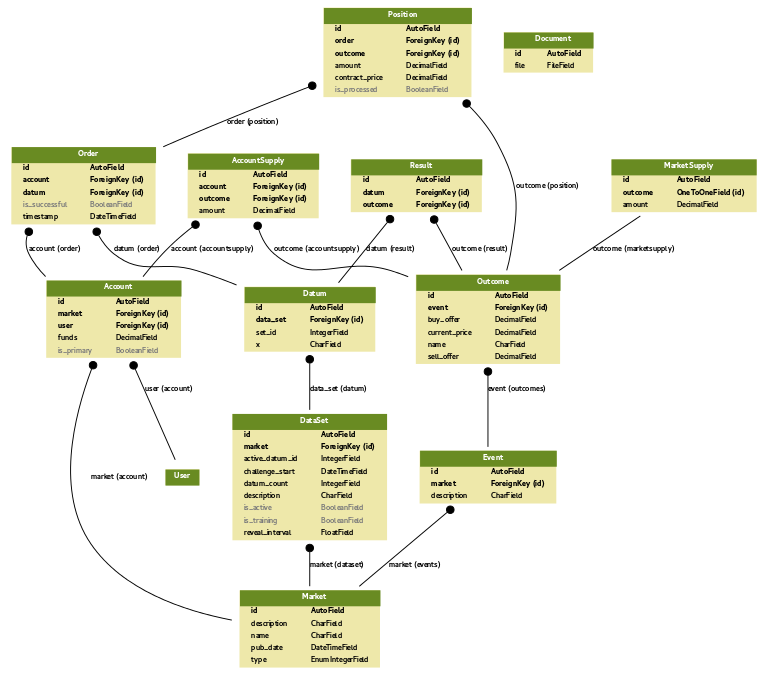
\includegraphics[scale=0.7]{figures/markets_graph.png} }
\label{fig:class-diagram}
{Legend: This is the class diagram showing the models comprising the market core. *Maybe talk about the composition of the diagram; how the different components are connected and interact with each other*}
\end{figure}
    
\section{Market Makers}
% talk about the market makers that were or can be implemented.
    What follows is an overview of the created market maker interface and the pricing algorithms investigated in the scope of the project.

\subsection{Interface}

The fundamental responsibilites of each {\em Market Maker} consist of the processing of incoming orders and the elicitation of current prices for the traded goods. Depending on its type, a {\em Market Maker} may also provide price quotes for orders instead of instantly processing them. Moreover, observe that the current prices change only when a new challenge is started, or when an order is processed. This makes it easy to introduce {\em signals} (a variant of the {\em Event} pattern in Django) within the implementation of these two methods, which in turn inform the underlying market maker and cause it to update the market state.  

Since the basic premise of the framework is the modelling of prediction markets we can assume that the process of resolving shares to rewards would be the same with every market maker. Namely we want to reward each agent with 1 credit for each share they own (and conversely deduct 1 credit for each share they own, if their position is short). This common functionality is implemented as part of the basic {\tt MarketMaker} class in a straightforward manner. 

{\tt end\_challenge}

The aforementioned requirements, as well as implementation of all common functionality, are defined in the {\tt MarketMaker} class. Note that Python does not support interfaces or abstract classes (the typical way of defining class responsibilities or protocols) which means that the required members are ordinary functions which should be overrided in derived classes, or throw exceptions otherwise. 

\subsection{Cron}

\subsection{Order Book}
    
    The “city plaza” market scenario where potential buyers and sellers place their offers and the matching ones are resolved. There is normally more than one way to complete trades where for example an agent sells at a price lower than that of a matching buyer, or an agent wishes to buy a larger quantity than a seller has to offer. Usually the market maker is neutral towards both the goods and their prices, but can also be made active by e.g. resolving arbitrage opportunities in his favour.

    Although they are simple to implement and operate, auctions of this type tend to create thin markets with volatile prices and low liquidity of the assets being traded. We can furthermore use the concept of Nash Equilibria to show that such markets do not incentivise players to share their true beliefs and are thus not well suited for model estimation (Myerson et al. 1983). Consider for example a buyer who values a given good well above its current market price: he or she would have no incentive whatsoever to let others (“the market”) know about their high valuation of the good but will instead seek to make trades at the lower price.

	Although listed first and arguably the simplest, {\bf Order Book} makers were implemented after the completion of the {\em Log-MSR} market maker. Particularly, since such markets are strictly neutral towards the traded goods and thus less flexible than other types of market makers, I decided they would not fully [exploit the capabilities of the framework]. 

    
\subsection{Parimutuel Betting}
This is the system usually used in gambling on sporting events, or in various lotteries. In it all bets of a type are put together in a pool, and the instantaneous odds are determined by the ratios between the already placed bets. The final winnings are determined by sharing the pool (minus any house cuts) amongst the winning bets. Even though they are easy to implement and operate, such markets do not offer any guarantees on the amount that is won in case of success (i.e. the final odds) since the latter is not known until all bets are collected.

This is the only one of the three market makers which was not written in code. 
[TODO: Move to Future Work along with another type of market which could be implemented]

\subsection{Market Scoring Rule}

In a market scoring rule (MSR) prediction market agents report a probability estimate r on the outcomes of an event and are rewarded sci(r) when outcome i happens. Proper scoring rules are rules which are monotonically increasing and thus reward estimates close to the truth the highest and penalise estimates that deviate from it. Proper scoring rules incentivise players to act according to their true beliefs.

	An example being the logarithmic market scoring rule (log-MSR) first proposed by Hanson in 2002 \cite{hanson_logarithmic_2002}. It is a proper (i.e. monotonically increasing) scoring rule which quantifies the risk (equivalently the self-information from information theory) assumed by the current stake, or position, of the market maker in this good. 

	Suppose we take an event $e$ with an outcome space $\omega_e$. Suppose also that for each type of share (and thus outcome) $o$ the current position of the market maker is given by $pos(o)$. The cost function is then given by:
$$C(e)=b*log(\sum_{o \in \omega} {e^{pos(o)}})$$

	Participants are subsequently charged according to the change in risk their positions incur. In practice this means that players who move the market prediction towards the {\it true} distribution get rewarded for doing so, while those who degrade the market prediction are penalised.

	


\section{Admin Interface}


    The admin interface is the place where the market operator or owner can create and configure the hosted markets and manage their state and contents in terms of events and data sets.

    Since the default installation of the framework comes with the built-in {\tt django-admin} module which serves this exact purpose, implementing the admin interface was considerably straightforward. Thanks to it most of the common or repetitive operations involving models (e.g. create, read, update, delete or CRUD) were purposefully easy to implement and configure. On the other hand, other less ``popular'' features, such as the option to pre-fill a dataset with randomised entries or to create both an event and its associated outcomes in one go, required carefully reading through the (often quite extensive) documentation. The admin module also provides a built-in user authentication system working on top of the existing Django user infrastructure which makes the writing of user-specific code similarly easy. 

\begin{figure}
 \caption{The index page of the administration interface. }
  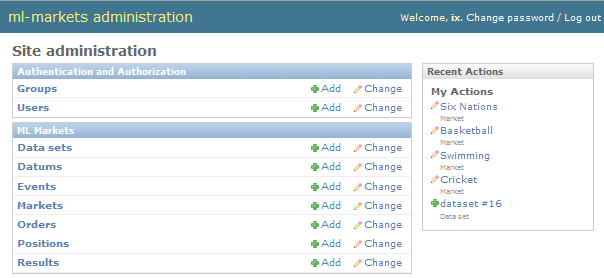
\includegraphics[width=\textwidth]{figures/admin-index(c).png}
   \label{fig:admin-index}
{This is the index page of the administration interface. The interface allows the administrator to authenticate and authorise the current participants in the market -  groups and users. The administrator also has an access to the components comprising the ML market. The administrator can both add new entries and edit existing ones.}
\end{figure}

	Figure \ref{fig:admin-index} displays the index page of the administration zone, accessible through the {\tt /admin/} URL. Its final look is largely the same as the original template used with every Django distribution, except for the changed title. This is to say that although it offers full functionality and looks fairly elaborate, the admin interface does not include any functionality which exceeds the capabilities of the framework. 

	As visible in Figure \ref{fig:admin-index}, the admin interface is structured in sections corresponding to the individual {\it models} accessible from it. Within code this is achieved by introducing special classes that derive from the base {\tt AdminForm} prototype, and are linked to each of the said models. Each class in turn specifies the fields and operations that can be accessed or modified by administrators, and allows the handling of particular events of interest related to the admin interface. As a Django convention all such objects must be declared in the {\tt admin.py} file within the {\tt markets} project. 

	The main functionality that the admin interface provides is the creation, modification and deletion (i.e. CRUD operations) of {\it markets}, {\it events} and {\it data-sets}. As shown in Figure \ref{fig:class-diagram} though, the last two of these models are in turn comprised of other objects, i.e. events with their possible {\it outcomes} and data-sets with the underlying {\it data} and the {\it results} of each datum. 

\subsection{Market Admin}

	Even though the {\it market} model is arguably the central and most important model in the created software, it is quite uncomplicated in the functionality or the members it provides on its own (for a discussion see Section \ref{sub:market}).  


\begin{figure}
\caption{Dataset actions}
 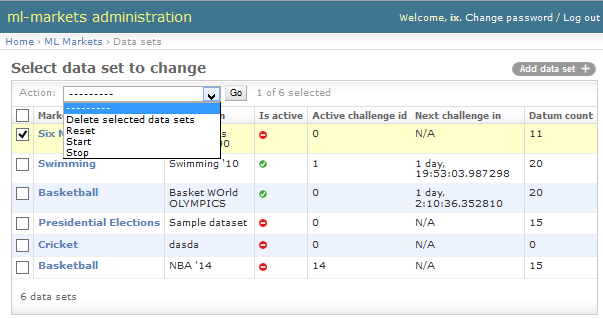
\includegraphics[width=\textwidth]{figures/admin-dataset-actions(c).png}

\label{fig:dataset-actions}
{This figure shows the {\it Data sets} menu accessible from the {\it Home} page of the {\it ml-markets administration}. The administrator can delete, reset, star or stop selected datasets. In addition, the administrator can also add new datasets, without the need to go back to the  {\it Home} page. The {\it Data sets} menu also provides brief desciption regarding the contents of the dataset, whether there is an active challenge involving the dataset in question and its {\it id}. The {\it Data sets} menu also shows when a next challenge is due to start, the starting date and time of the last challenge and the datum count in the data set.} 
\end{figure}

\begin{figure}
\caption{market actions}

\begin{subfigure}{.8\textwidth}
  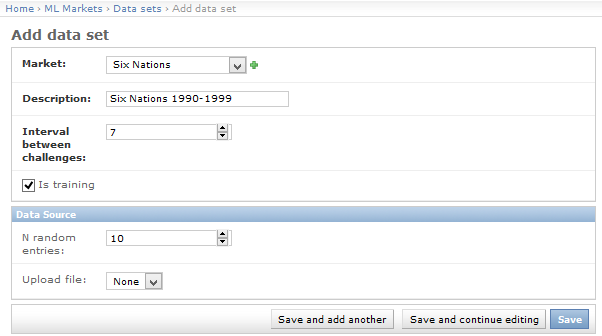
\includegraphics[width=1\linewidth]{figures/admin-dataset-add(c).png}
  \caption{add dataset}
   \label{fig:add-dataset}
\end{subfigure}%

\begin{subfigure}{.8\textwidth}

  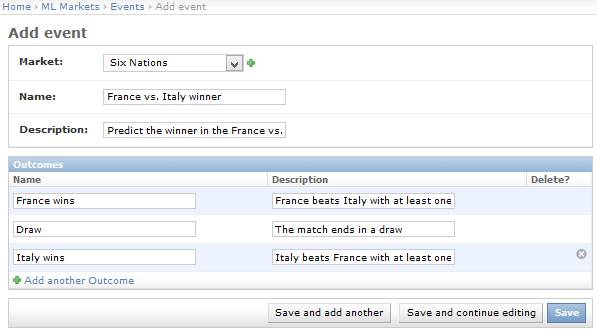
\includegraphics[width=1\linewidth]{figures/admin-event-add(c).png}
  \caption{add event}
  \label{fig:add-event}
\end{subfigure}

\begin{subfigure}{.8\textwidth}

  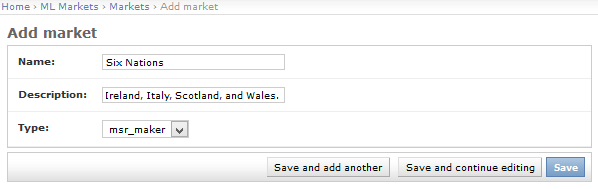
\includegraphics[width=1\linewidth]{figures/admin-market-add(1).png}
  \caption{add market}
  \label{fig:add-market}
\end{subfigure}
\label{fig:market-actions}

{This figure shows examples of different {\it Market actions} available from the {\it Home} menu of the {\it ml-markets administration}. Addition of new {\it data sets}, {\it events} and {\it markets} are used as representative examples. Panel a) Add data sets: The administrator can select, using a drop-down menu, to which market to add the new {\it data sets}. The menu allows the administator to enter the {\it data set} desciption and to select the interval between the challenges involving the new {\it data set}. The administrator can also indicate whenther the new {\it data set} is used for training. The {\it Data Source} tab allows the administrator to upload a new file and to select the number of random entries. Panel b) Add event: The administrator can use drop-down menu to select a {\it market} with which to associate the new event. The administrator cal selects a {\it name} for the event and add {\it description}. The {\it Outcomes} tab allows administrators to enter {\it name} and {\it desciption} for each {\it outcome}. Addition of new {\it outcome} is straightforward, using a button conveniently located at the bottom of the list with existing outcomes. Panel c) Add market: The administrator can add new {\it markets} and enter {\it name} and {\it desciption}. Using a drop-down menu, the administrator can select the {\it type} of the market.}  
\end{figure}



[TODO: alot more]
\section{User Interface}
% mention the static interface, js graphics !!

\begin{figure}
\caption{User login and index}
\begin{subfigure}{.5\textwidth}

  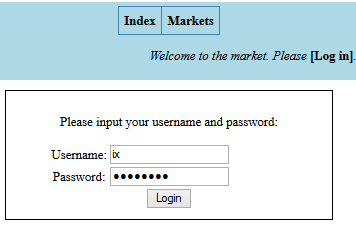
\includegraphics[width=.95\linewidth]{figures/ui-user-login(c).png}
  \caption{user login}
  \label{fig:ui-user-login}
\end{subfigure}%
\begin{subfigure}{.6\textwidth}

  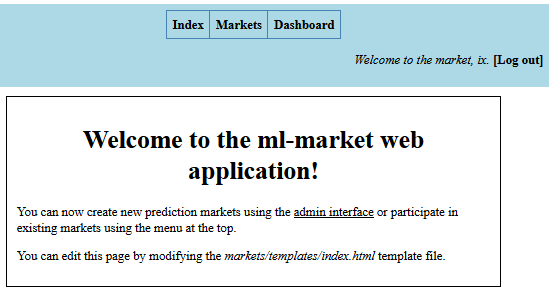
\includegraphics[width=1\linewidth]{figures/ui-index(1).png}
  \caption{index}
  \label{fig:ui-index}
\end{subfigure}
\label{fig:ui-login-index}
{add legend here}
\end{figure}

\begin{figure}
\caption{Market list and market index}

\begin{subfigure}{1\textwidth}

  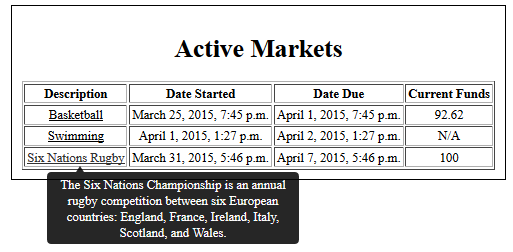
\includegraphics[width=1\linewidth]{figures/ui-market-list(c).png}
  \caption{market list}
  \label{fig:ui-market-list}
\end{subfigure}%

\begin{subfigure}{0.6\textwidth}
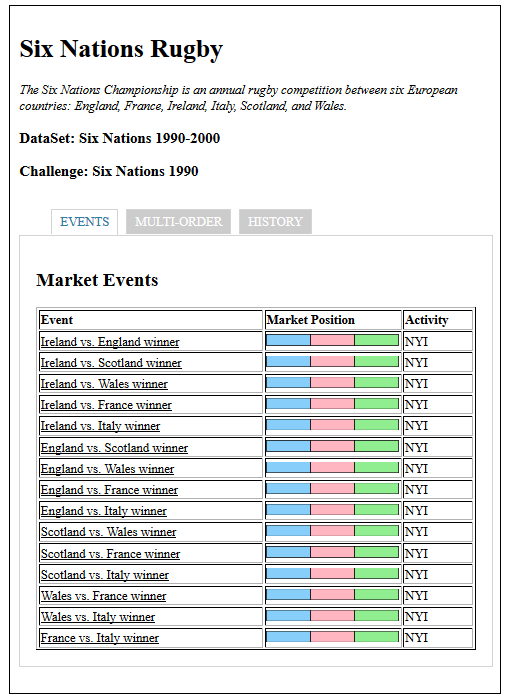
\includegraphics[width=1\linewidth]{figures/ui-market-index(c).png}
  \caption{market index}
  \label{fig:ui_market_index}
\end{subfigure}
\label{fig:market-list-index}

{add figure legend here}
\end{figure}





	As Django follows the MVC architectural pattern, it defines three major component types that control the flow of information from and to the user: the models, views, and controllers. We already examined the models which comprise the back-end market structure in Section 5.3. In this section I talk about the components which shape and define the overall user experience. 


	Similarly to the admin module, the UI must support a number of fundamental operations such as performing user authentication, and providing limited model interaction capabilities. 


On the other hand there is much in the way information is presented on the screen, and the different visualisations that help a user grasp the current market position and dynamics. While the Django framework comes equipped with a number of modules that greatly simplify generic tasks such as the ones above, the problem of designing an {\em informative} and [TODO] market is one that [deserves a project on its own]. There are a number of studies examining the role of user interfaces for prediction markets ([TODO: cite]) but implementing a real-time [informative, visual interface for real would be way too time-consuming]. 


    Due to my limited abilities in html and javascript the current user interface is fairly simple. Apart from basic features such as (secure) user registration and login, it provides price quotes and transaction history for markets. There are a few directions I would like to expand on: for example by including histograms to visualise the prices or the trade volume in a market, by allowing browsing other agents’ portfolios, and making the interface more intuitive as a general. A great case study is presented in “A Combinatorial Prediction Market for the U.S. Elections” by Dudik et. al

\subsection{Authentication}

	Django comes with a flexible, built-in user authentication system. Its most notable features include the support of user groups and permissions, basic registration and log-in forms, as well as different authentication and password policies. While these features significantly reduced the amount of {\it boilerplate} code I had to write, the last of those was of special interest to me as I have (first-handedly) found it is surprisingly easy to introduce security vulnerabilities, even when implementing relatively simple and well-known concepts such as password encryption or salting. 



	


\subsection{Views}
	The views blahblah

Talk about request format, types, 

input verification: betting data, user handling; lack of challenge-id-check-when-bet

\subsection{Forms}
	The concept of {\bf Forms} in Django (also the ``C'' in its MVC architecture) derives directly from the concept of {\em HTML forms} used for implementing operations such as {\tt GET} or {\tt POST}. Written in Python, their purpose is to simplify many of the common operations related to HTML forms and the handling of user input in general, such as establishing connections to existing back-end models, performing validation, or preparing the fields of a model for rendering. 


\subsection{Templates}
 Talk about how I implemented the HTML templates. 

\subsubsection{Static Files}
Talk about the static files: CSS, JavaScript
	The static files include the style-sheets used throughout the site and the various front-end JavaScript functions I wrote as part of the user interface. 

	Due to a number of concerns I adopted the common practice of separating the structure of the user-facing code from its design by the use of external style-sheets. This was done in order to emphasize the flexibility of the interface, but also to allow the use of the same style-sheets across different pages. 

	

\section{API}
    
    Implementing a remote API was one of the more important features of the project in in terms of its intended use as a prediction market framework. Its basic premise is to allow for the development of automated agents that interact with existing markets. While in theory most, if not all, of its functionality mirrors that of the user interface, it is important that the API operates in a secure, well-defined fashion.
    
    I first approached the problem by trying to manually write the handlers for API requests. This did not go as planned as I had not considered that most, if not all, of its functionality is the same as the functionality offered by the underlying models and views 

\section{Other Tools}

\subsection{django-extensions}
    This package is an MIT-licensed collection of extension tools which ease the process of developing Django apps. The two most useful features I used were the ability to automatically generate {\tt django-admin} templates and GraphViz {\tt dot} files of the models in a package. 

\subsection{Sphinx}
    Sphinx is a flexible documentation generator which converts {\tt reStructuredText} (reST) files to a number of formats, most notably PDF and HTML. ReST is a flexible markup language widely used for documentation purposes in the Python community. I was not initially supportive of the idea of learning yet another markup or template language but after looking at possible alternatives Sphinx looked like the most reliable, widely used and {\em pythonic} solution out there. In the end I was able to both quickly generate automatic documentation from the code, and then manually extend and insert additional explanations and use cases for the examples in question.

\section{Testing and Documentation}
% documentation at github.io ?!
% issue tracker ?!?!
% wiki too ?!?!?!?
    When it comes to designing and testing an application dealing with any kind of transactions, it is clear that a set of minimum requirements has to be met in terms of consistency and transactional integrity. Fortunately the high-level nature of the language and the framework make this straightforward.

I initially wanted to adopt a test-driven approach towards the development process but doing so proved problematic for the first few months of the project. During this time I was initially modelling the market structure and later writing code for the user and admin front-ends. Most of the work was thus of declarative nature and there were a limited number of non-trivial unit tests that I could come up with. On the other hand, as Python makes writing runtime validation code (i.e. assertions) incredibly easy, I used this feature extensively since the beginning of the project as a way to complement existing in-code documentation and unit tests. 

I approached the question of creating documentation in a similar manner to testing, relying on in-code documentation in the form of {\em docstring} comments for most of the development process. Then, once I had more-or-less finalised the model designs, I added custom sections with explanations better suited to the individual components. 

\subsection{Unit Tests}

    The main body of unit tests deals with the core market structure and does verification of the basic mechanisms underlying the markets. Example tests include starting, stopping and resetting a dataset or checking if the ``Cron`` module properly dispatches signals whenever markets expire. 
    I took a similar approach when writing the tests for the implemented market maker modules. Currently there are tests only for the {\tt msr-maker} as the other available maker - the order book - is completely neutral. 

[TODO: table with unit testa and their status]
    
\subsection{Runtime Tests}
    
    The code features a multitude of runtime tests checking model invariants. For example, the joint asset prices for an outcome space always summing to 1 is enforced throughout the market makers, but there are also explicit checks executed every time prices change.

    While designing the base models, I paid extra attention to transactional atomicity: it would be quite inappropriate if funds appeared or vanished while serving requests in a market. Thankfully the framework allows for fine and idiomatic control of transaction lifetime using method decorators and ``with`` blocks.

[TODO: introduce examples, talk about usefulness in practice]

\subsection{Documentation}

    The documentation is an integral part of the life-cycle of any software which pretends to be extensible and maintainable, and is especially true in the case of frameworks. While most of the existing documentation is generated automatically, 
    
\subsection{Issues}
    [TODO: go over existing issues, the tracker]
    
\chapter{Evaluation and Reflection}

This chapter includes evaluation of the completed project and reflection on the possible use cases of the software. 

\section{Software Evaluation}

\subsection{Functionality}

\subsection{Interface}


\section{Reflection and Use Cases}
% The original project was named ... and involved ... My analysis showed that ... may be too much and instead a frameworkish report might be better

\subsection{Prediction Markets}

\subsection{Model Aggregation}

\subsection{Crowdsourced Machine Learning Contests}

\chapter{Conclusion}
% prediction markets and how they can be improved to do even better job
% useful scenarios (e.g. election results, cancer cell detection etc).
% “powerful tool for…”, “excellent alternative to current techniques”




% use the following and \cite{} as above if you use BibTeX
% otherwise generate bibtem entries
\bibliographystyle{unsrt}
\bibliography{ixlib}

\end{document}

